% !TEX root = ../EDBT.tex
\begin{figure}
\centering
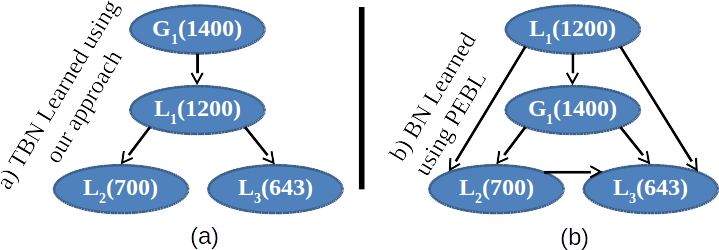
\includegraphics[width = 100mm]{Figures/g1Network.png}
\vspace{6pt}
\caption{Structure learned of $G_1$ using two different approaches}
\label{fig:g1net}
%\vspace{-10pt}
\end{figure}

We present the accuracy of our predictions on a real-life dataset from a global market research organization. We set a threshold $\tau$ on CoP, and predictions with a CoP $< \tau$ are routed for human annotation. We also measure the accuracies of our predictions for different values of $\tau$.

\textit{\textbf{Data description}}: We have data for carbonated drinks of $26$K unique products from a single geography, contained in two datasets:
a)~\textbf{Local DB}: It contains 26K products with each product having $49$ local characteristics, where cardinality of local characteristics varies from tens to thousands. It also contains descriptions of products given by retailers of that product, where number of descriptions of a single product varies from tens to hundreds. b)~\textbf{Global DB}: It contains four global characteristics with cardinality varying from tens to thousands.

\textbf{\textit{Data Preparation:}} We predict four global characteristics $G_1$, $G_2$, $G_3$, and $G_4$ for two cases, with varying ratio of split between training, validation and test datasets. \textbf{\textit{Case-1}}(60:20:20) has 60\% training, 20\% validation and 20\% test and \textbf{\textit{Case-2}} has this ratio as 20:20:60. \textbf{NOTE:} While Case-1 uses a traditional split of training vs testing data, Case-2 is more realistic, since in practice preparing a training data by manual data labeling is costly: For example, we would like to `onboard' a data from a particular dataset 
by manually annotating only a small fraction (e.g. 20\%) of records and automate the remainder or we might like to board 
data from one organization (e.g. retailer or distributor) in a particular geography in the hope that data from remaining sources in that
geography share similar local characteristics, eliminating manual annotation for a large volume of data. 
To simulate this practical scenario, we used the first few records from the local dataset, which happened to contain only 10\% or so of the
total possible values of each global attribute.

For SBM, $\eta$ relevant local characteristics was chosen for every $G_j$. Figure~\ref{fig:g1net}, compares the Bayesian network structure learned using our approach and another learned using an open source python library Pebl \cite{shah2009python}, for the global characteristic $G_1$. Clearly, network obtained using Pebl (Figure~\ref{fig:g1net}(b)) is more complex as compared to ours \ref{fig:g1net}(a), as the size of CPTs of these are of the order of a)~$1200\times1400$ and b)~$1200\times1400\times700\times643$ respectively. %Scaling factor $\lambda=0.1$ was used in Equation~\ref{eq:soft} for predictions using UTS model.

\begin{figure}
\centering
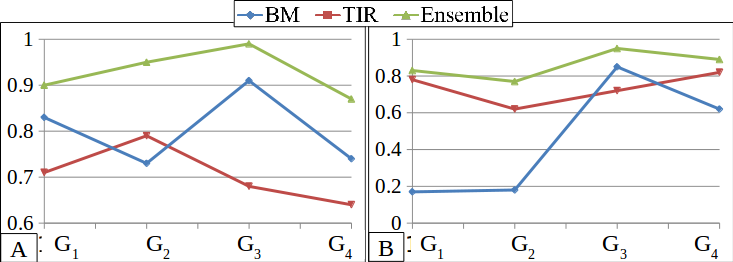
\includegraphics[width= 90mm]{Figures/Case1-2.png}
%\vspace{-10pt}
\caption{x-axis: global characteristics, y-axis: A)~Predictive accuracy for Case-1, B)~Predictive accuracy for Case-2}
%\vspace{-8pt}
\label{fig:case-1}
%\vspace{-8pt}
\end{figure}

Figure \ref{fig:case-1}, shows the prediction accuracy of four global characteristic for Case-1 and Case-2 respectively. Here, the accuracy is a ratio of correctly predicted products to the total number of products. In Case-1, accuracy of Ensemble model is in the range of 85 to 99\%  and it outperforms both SBM and UTS for all four global characteristics.

\textbf{\textit{Baseline Comparison}}: We also compared our approach with record matching method implemented in a framework called FEBRL\cite{christen2008febrl}. For attribute matching, we tried three similarity measures winkler, tokenset, trigam and show the results with winkler which outperforms the rest. We tested this approach for the Case-1 on the smaller dataset (5K products). Table~\ref{table:comparison}, shows the comparison of the prediction accuracy of four global attributes using our Ensemble approach and FEBRL. This suggests that our approach outperforms and also shows that accuracy of FEBRL decreases for high cardinality global attributes. FEBRL did not work on, 26k products, on a machine with 16GB RAM, Intel Core i7-3520M CPU 2.90GHz* 4, 64 bit. We did not try the blocking method as main motive of our problem is to improve accuracy of prediction, and not the time complexity. 
\renewcommand{\arraystretch}{}
\begin{table}
%\scriptsize 
  \centering
  %\small
  \begin{tabular}{|c|c|c|c|} 
   \hline
   Global att. & Num of states & FEBRL(winkler) & Ensemble \\
   \hline
   $G_1$ & 107 & 86\% & 93\% \\
   \hline
   $G_2$ & 154 & 57\% & 95.2\% \\
   \hline
   $G_3$ & 3 & 99.3\% & 99.2\% \\
   \hline
   $G_4$ & 13 & 95.4\% & 99.4\% \\
   \hline 
  \end{tabular}
  %\vspace{4pt}
\caption{Comparison of our approach with FEBRL}
  \label{table:comparison}
  %\vspace{-15pt}
\end{table}
\textbf{Case-2} (Figure \ref{fig:case-1}-B), naturally renders the SBM less accurate, since the training data contains only 10\% of possible states of each global characteristic. However, it is compensated by the performance of UTS, which searches the target set of global attribute values from the
retailer descriptions. Combining these models using our Ensemble model the accuracy of four global characteristics reaches 78 to 93\%.

\textbf{\textit{CoP Threshold for human annotation:}} We define three categories: a)~\textbf{P-C:} Number of products \textit{predicted correctly} by our approach for which CoP $> \tau$. b)~\textbf{P-I:} Number of products \textit{predicted incorrectly}, for which CoP $> \tau$. c)~ \textbf{NP:} Products which we choose \textit{not to predict}, i.e., products with CoP $\leq \tau$. We select $\tau$ in order to maximize P-C and minimize P-I category, while not increasing NP so much that exercise becomes almost entirely manual. Since products in the P-I category are more costly for a company as compared to NP category, we give more weight to P-I while learning $\tau$. Table~\ref{table:categories}, shows the percentage of products in each category (P-C, P-I, NP) on validation set along with the threshold $\tau$ values for both cases. It shows that for given $\tau$, percentage of products in P-C category is in the range of 81-96\% for Case-1, whereas, it ranges from 70 to 96\% for Case-2. Also, the average percentage of products in P-I category is only around 5\%. These numbers establish that CoP is a good measure for reliability of predictions. Figure~\ref{fig:PC-2}, shows the variation in the percentage of products in test set of each category with respect to threshold value $\tau$ for both Case-1 and Case-2, for the global characteristic $G_1$. It validates the optimal values of $\tau$ learned using validation set, 0.5 for Case-1 and 0.6 for Case-2.

The process of aggregate analysis, comparing global market share and sales of product categories is carried out in our platform \textbf{\textit{iFuse}}\cite{singh2016visual} (Figure~\ref{fig:iFuse}). Figure~\ref{fig:iFuse}(a),(b) shows the data tile and cart view of iFuse representing the attributes of the local DB and global DB to be linked together. Figure~\ref{fig:iFuse}(c) shows the tile view of the attributes obtained after mapping of local DB to global attribute, here GLO BRAND via ensemble approach, thereby enabling the \textbf{join} of local sales and global market share via common global attribute, GLO BRAND (Figure~\ref{fig:iFuse}(d)). Figure~\ref{fig:iFuse}(e) shows aggregate analysis of different products via motionchart.

\renewcommand{\arraystretch}{}
\begin{table}
  {%\scriptsize
  \centering
  \begin{tabular}{|p{0.7cm}|c|c|c|c|c|c|c|c|}
    \hline
    \multirow{2}{*}{Global} &
      \multicolumn{4}{c|}{Case-1} &
      \multicolumn{4}{c|}{Case-2} \\
      \cline{2-9}
    & $\tau$ & P-C & P-I & NP & $\tau$ & P-C & P-I & NP \\
   \hline
   $G_1$ & 0.5 & 92\% & 4\% & 4\% & 0.6 & 82\% & 7\% & 11\% \\
   \hline
   $G_2$ & 0.6 & 81\% & 7\% & 12\% & 0.65 & 74\% & 10\% & 16\% \\
   \hline
   $G_3$ & 0.7 & 96\% & 1\% & 3\% & 0.7 & 96\% & 1\% & 3\% \\
   \hline
   $G_4$ & 0.8 & 86\% & 3\% & 11\% & 0.8 & 85\% & 4\% & 11\% \\
   \hline
  \end{tabular}
  %\vspace{4pt}
  \scriptsize
  \caption{\% of products in each category on Validation set}
  \label{table:categories}
  %\vspace{-7pt}
  }
\end{table}

%\begin{figure}
%\centering
%\includegraphics[width = 65mm]{Figures/PC-PI-NP}
%\vspace{-8pt}
%\caption{Percentage of Products in each category for different values of $\tau$ on test data for $G_1$ in Case-1}
%\label{fig:PC-1}
%\vspace{-10pt}
%\end{figure}
%\vspace{-5pt}
\begin{figure}[!t]
\centering
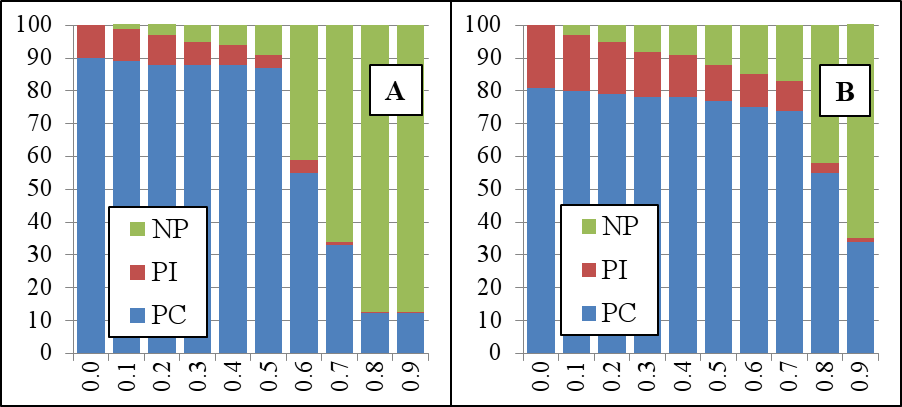
\includegraphics[width=100mm]{Figures/Fig67.png}
%\vspace{4pt}
\caption{\% of Products in each category for different values of $\tau$ on test data for $G_1$ in A)~Case-1 and	 B)~Case-2}
\label{fig:PC-2}
%\vspace{-14pt}
\end{figure}
\begin{figure}
\centering
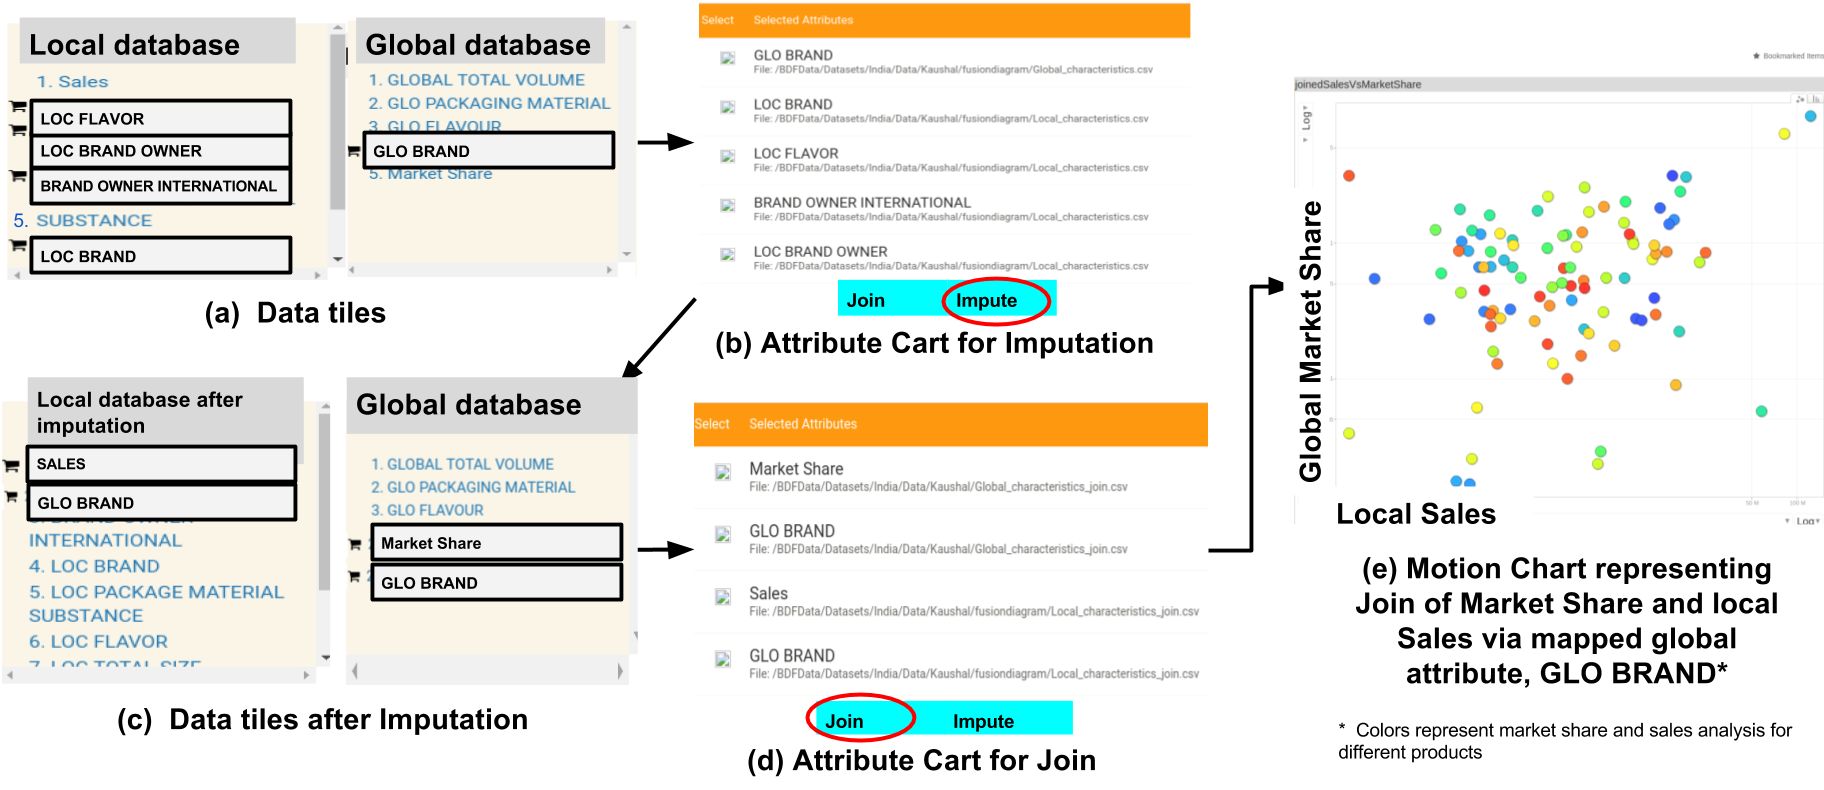
\includegraphics[width = 120mm]{Figures/EDBT_diagram3.png}
%\vspace{-8pt}
\caption{Figure showing aggregate analysis of global market share and local sales done using our platform. }
\label{fig:iFuse}
%\vspace{-12pt}
\end{figure}

% \begin{figure*}
% \centering
% \includegraphics[width=80mm]{Figures/iFuse}
% \vspace{1pt}
% \caption{jdd}
% \label{fig:iFuse}
% %\vspace{-16pt}
% \end{figure*}